\documentclass[margin,line]{resume}

% \definecolor{sidebarcolor}{RGB}{204, 153, 0}
\definecolor{sidebarcolor}{RGB}{189, 155, 50}
% \definecolor{sidebarcolor}{RGB}{203, 172, 70}

\usepackage[utf8]{inputenc}
\usepackage[english,russian]{babel}
\usepackage[T1]{fontenc}
\usepackage{fontawesome}

\begin{document}

{\vspace*{-13mm}\sc \large Гришин Антон — Go разработчик} \\
\begin{resume}
  \begin{minipage}[t]{0.55\textwidth}
    \section{\mysidestyle Персональная\\Информация}
    Москва, Россия \\
    \faGithub  \space
    \href{https://github.com/alchemmist/}{\texttt{alchemmist}} \\
    \faLinkedin \space
    \href{https://www.linkedin.com/in/anton-grishin-6966a8362/}{\texttt{anton-grishin}}
    \\
    \faPaperPlane \space \href{https://t.me/alchemmist}{\texttt{@alchemmist}} \\
    \faPhone \space
    \href{tel:+1234567890}{\color{blue}\texttt{+7(915)067-2638}}  \\
    \faEnvelope \space
    \href{mailto:anton.ingrish@gmail.com}{\color{blue}\texttt{anton.ingrish@gmail.com}}
  \end{minipage}

  \begin{minipage}[H]{0.18\textwidth}
    \begin{textblock}{7}(10.96, 1.30)
      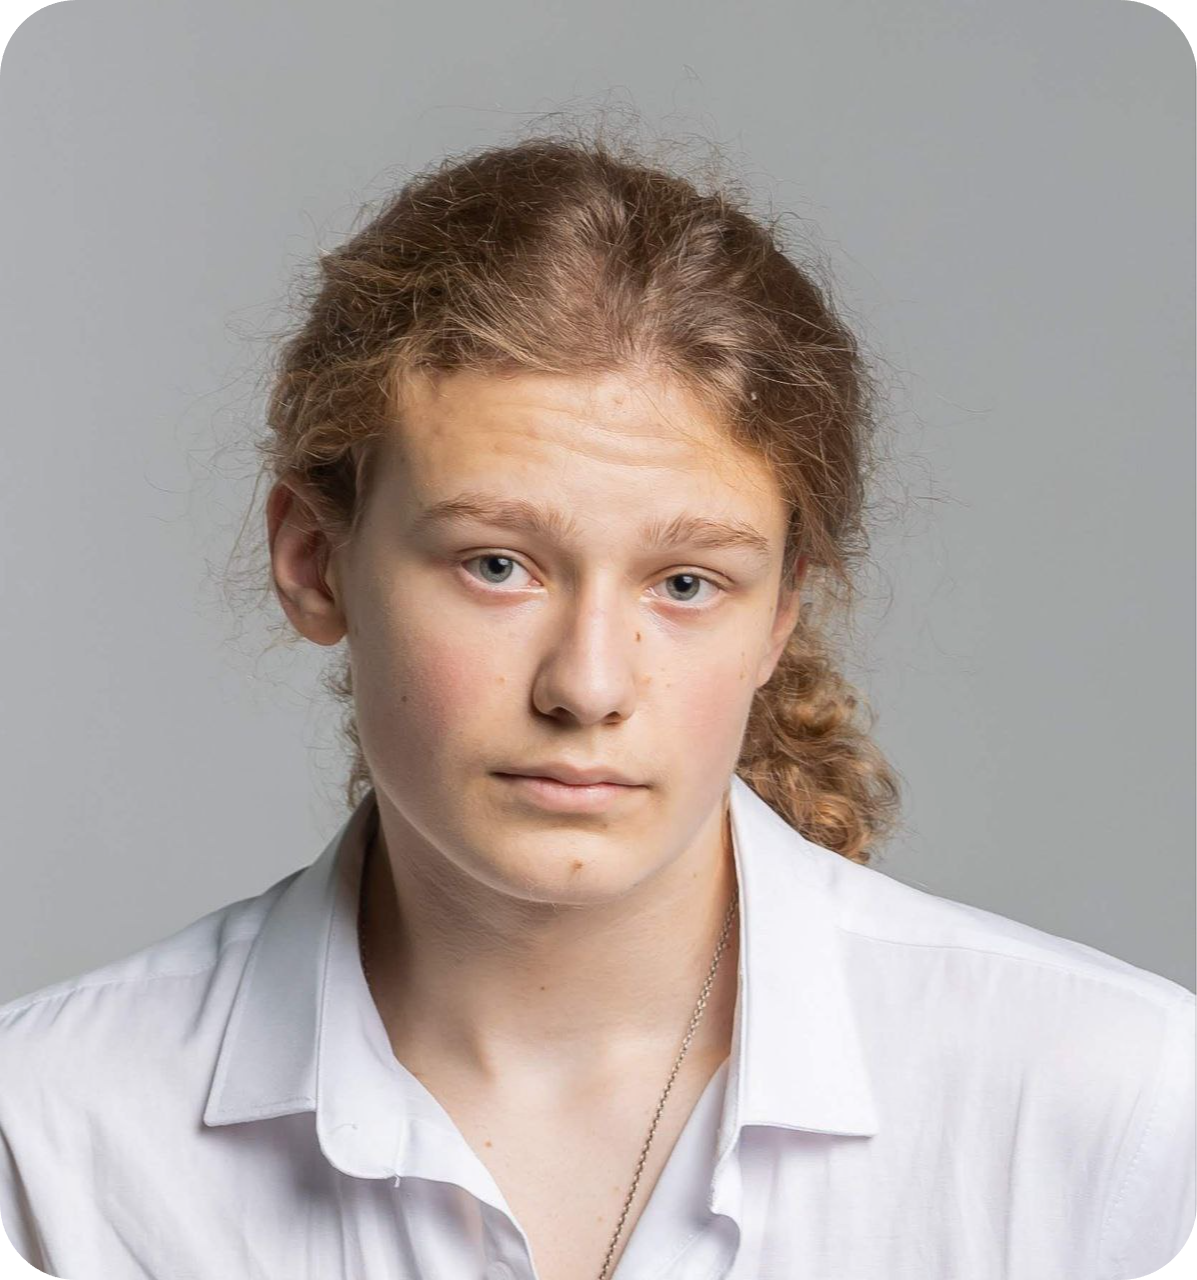
\includegraphics[width=0.255\textwidth]{../images/avatar.png}
    \end{textblock}
  \end{minipage}

  \vspace{-7mm}
  \section{\mysidestyle Обо мне}
  Я студент, начинающий разработчик. Программирую 4 года, за
  это время участвовал в разработке 44 репозиториев, отправил 921
  коммит и написал 176729 строчек кода.
  \href{https://www.avito.ru/moskva/predlozheniya_uslug/prepodavatel_programmirovaniya_na_python_2556461612}{Преподаю}
  Python, обучил $> 30$ учеников. Сооснователь и
  разработчик в \href{https://ballkit.ru/}{Баллкит}. В прошлом профессиональный
  \href{https://alchemmist.github.io/CV/attachments/sport.pdf}{волейболист}.

  \section{\mysidestyle Образование}
  \href{https://centraluniversity.ru/}{Центральный Университет} —
  Математика и компьютерные науки, 2028 \textit{(1 курс)}.
  Направление «Разработка». Траектория «Computer Science Research».
  % TODO: уточнить трек

  \section{\mysidestyle Навыки}

  \vspace{0.4mm}
  \begin{description}[leftmargin=0pt, itemindent=*, itemsep=0.2pt]
    \item[Go:] \inlinecode{http}, \inlinecode{grpc},
      \inlinecode{protobuf}, \inlinecode{tgbotapi},
      \inlinecode{reflect}, \inlinecode{gofsm}.
    \item[Databases:] \inlinecode{postgres}, \inlinecode{sqlite},
      \inlinecode{redis}, \inlinecode{Yandex Object Storage}.
    \item[Message brokers:] \inlinecode{RabbitMQ}, \inlinecode{Mosquitto}.
    \item[Other technologies:] \inlinecode{SQL}, \inlinecode{Java},
      \inlinecode{JavaScript}, \inlinecode{bash}.
    \item[Dev tools:] \inlinecode{Docker}, \inlinecode{Podman},
      \inlinecode{Make}, \inlinecode{CI/CD}, \inlinecode{Linux},
      \inlinecode{Git}
  \end{description}

  \section{\mysidestyle Достижения}
  Прошёл в
  \textbf{финал}
  (\href{https://alchemmist.github.io/CV/attachments/russian-chemp-final.pdf}{\texttt{1}})
  \href{https://events.fsp-russia.com/championship}{Чемпионата
  России} по спортивному
  программированию, среди 5000 участников. Разработал
  \href{https://alchemmist.github.io/CV/attachments/architect.pdf}{микросервисную
  архитектуру} из 9 сервисов для
  \href{https://github.com/alchemmist/sportprog}{веб-приложения},
  агрегирующего спортивные события по
  всей России. И разработал
  \href{https://github.com/alchemmist/sport-afisha/blob/main/event_parsing_service/parse_pdf.py}{алгоритм}
  обработки и проверки ежегодных
  государственных
  отчётов о спортивных мероприятиях. Технический стек:
  \inlinecode{Kafka}, \inlinecode{React},
  \inlinecode{RabbitMQ (FastStream)},
  \inlinecode{FastAPI},
  \inlinecode{OAuth}.
  % TODO: вложить хакатон на github и добавить ссылку

  \vspace{-6mm}

  \hfill \textsl{Декабрь 2024}

  \textbf{\href{https://alchemmist.github.io/CV/attachments/scince-for-life-win.pdf}{Победитель}
  научно-практической конференции}
  «\href{https://conf.profil.mos.ru/academ}{Наука для
  жизни}» среди 117 проектов с
  \href{https://github.com/smart-cab/}{проектом умного
  дома} для частных и государственных
  образовательных учреждений. Технический стек: \inlinecode{Redis},
  \inlinecode{Zigbee2MQTT}, \inlinecode{websockets}, \inlinecode{Go},
  \inlinecode{Python}, \inlinecode{Flask}, \inlinecode{React}.
  \vspace{-6mm}

  \hfill \textsl{Апрель 2024}

  \vspace{-2mm}

  \section{\mysidestyle Опыт}\vspace{2mm}

  \begin{description}

    \item[Patch Loyalty]\small Программа лояльности для малого бизнеса \hfill
      \textsl{Июль 2024 — Август 2024\vspace{1mm}}\\
      Разработал бота в Telegram по модели SMB (Single Message Bot) на
      \inlinecode{Go} для коробочной системы лояльности
      \href{https://ballkit.ru}{\texttt{ballkit.ru}}.

      \textbf{Технологии:}
      \inlinecode{Go},
      \inlinecode{tgbotapi}, \inlinecode{grpc},
      \inlinecode{gofsm}.
  \end{description}
  \vspace{-4mm}
  \section{\mysidestyle Интересы}\vspace{0.7mm}

  {\textbf{Формальная верификация:} Прохожу курс
    \texttt{\href{https://softwarefoundations.cis.upenn.edu}{softwarefoundations}}.
    Прочитал первый том,
    \href{https://github.com/alchemmist/coq-learning}{доказал} 250
  теорем на \inlinecode{Coq}.} \\

  \vspace{-6mm}

  \textbf{Linux:} Использую Arch с композитором Hyprland. Опубликовал
  свои
  \href{https:/github.com/alchemmist/.dotfiles}{\texttt{.dotfiles}}.
  С нуля написал свой Neovim
  \href{https://github.com/alchemmist/.dotfiles/tree/main/nvim}{конфиг}
  и цветовую
  \href{https://github.com/alchemmist/nothing.nvim}{тему}.
  Написал более 20 кастомных
  \href{https://github.com/alchemmist/.dotfiles/tree/main/scripts}{скриптов}.

  \end{resume}

  \begin{minipage}[H]{9.18\textwidth}
    \begin{textblock}{7}(-0.65, 15.1)
      \begingroup
      \hspace{35mm}
      \hypersetup{urlcolor=gray!90}
      \large
      \href{https://github.com/alchemmist}{→ больше проектов на
      \underline{GitHub}}
      \endgroup
    \end{textblock}

  \end{minipage}

  \clearpage

  \end{document}
